\documentclass[border={0.1cm -0.25cm 0.1cm 0.1cm}]{standalone}  %E,S,W,N
%\documentclass{scrartcl}

\usepackage{amssymb}
\usepackage{amsmath}
\usepackage{tikz}
\usetikzlibrary{arrows,arrows.meta}	%big arrowheads

\begin{document}
	
	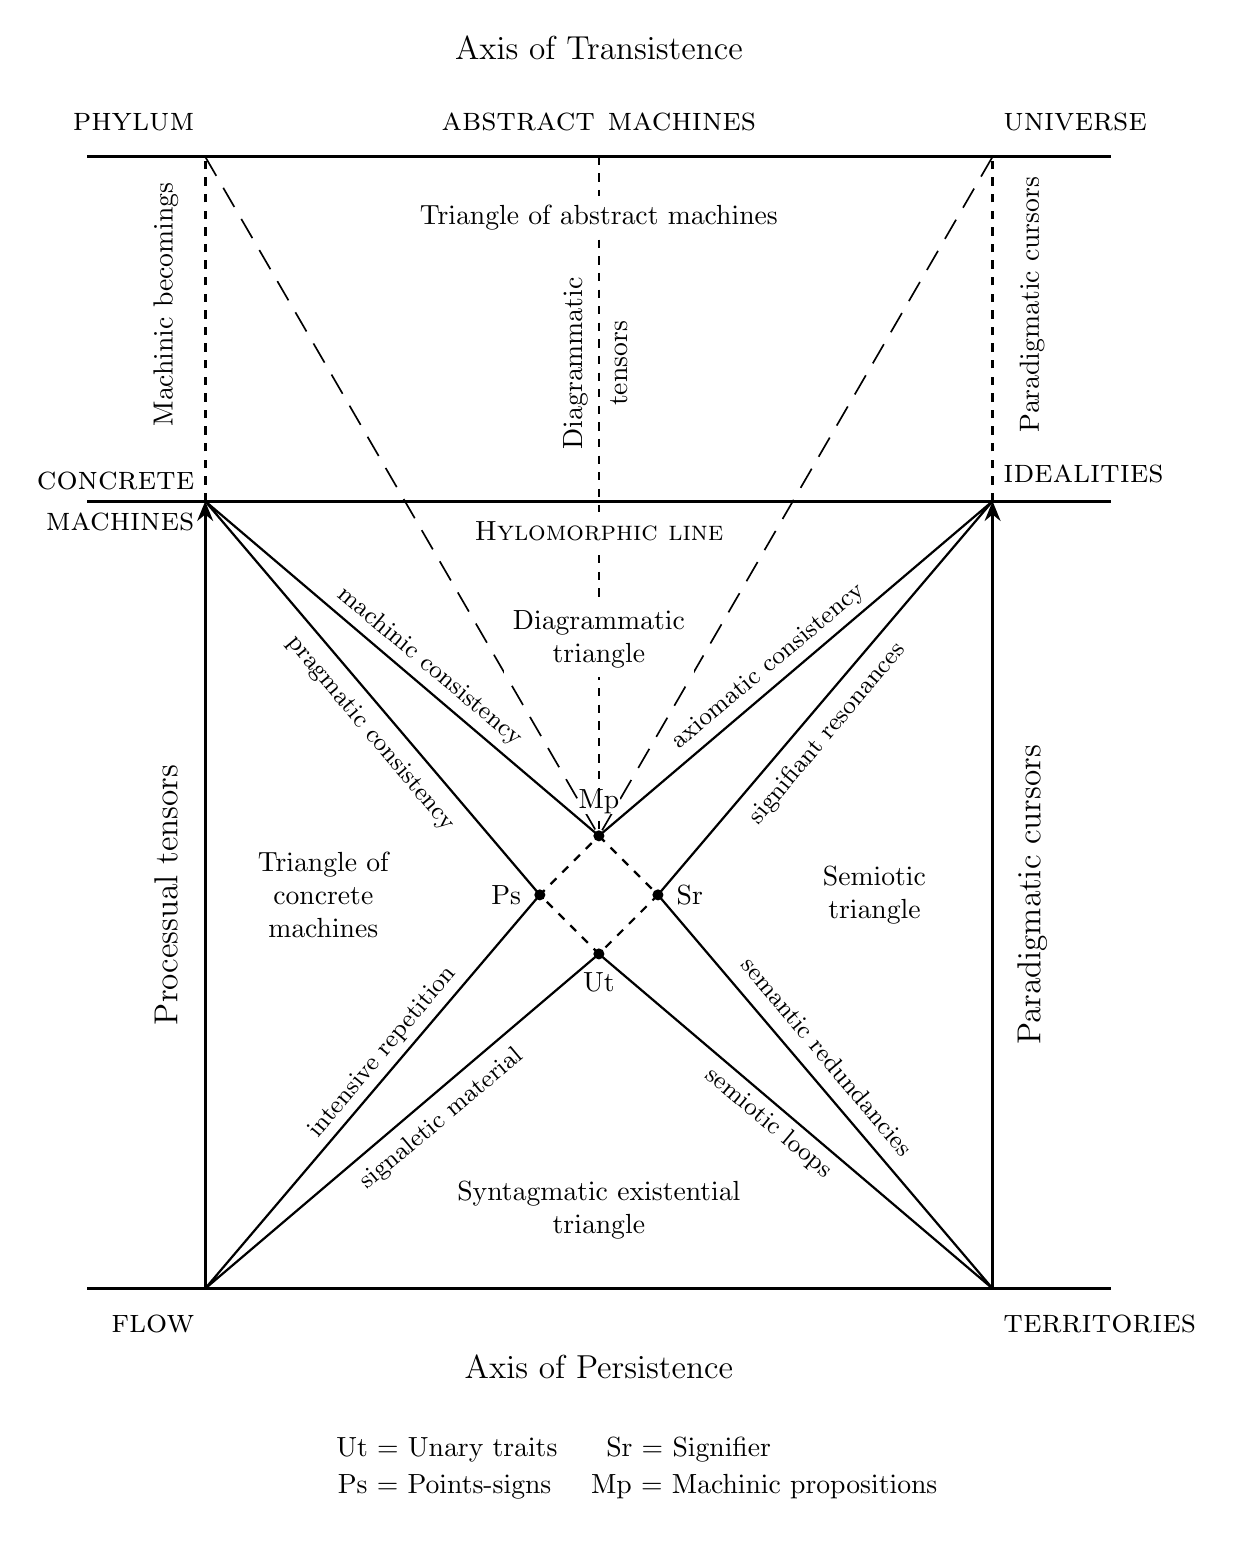
\begin{tikzpicture}[very thick]
	\def\s{5} %side of main square
	
	%MAIN SQUARE
	%\draw (-\s,\s)--(\s,\s)--(\s,-\s)--(-\s,-\s)--cycle;
	\draw (-1.3*\s,-\s)--(1.3*\s,-\s);
	\draw (-1.3*\s, \s)--(1.3*\s, \s);
	\draw (-1.3*\s,1.875*\s)--(1.3*\s,1.875*\s);
	%
	\draw[-{Stealth[length=2.5mm,width=2mm]}] (-\s,-\s)--(-\s,\s);
	\draw[dashed] (-\s,\s)--(-\s,1.875*\s);
	\draw[-{Stealth[length=2.5mm,width=2mm]}] (\s,-\s)--(\s,\s);
	\draw[dashed] ( \s,\s)--( \s,1.875*\s);
	%
	\draw[thick,dashed] (0,0.15*\s)--(0.15*\s,0)--(0,-0.15*\s)--(-0.15*\s,0)--cycle;
	\draw[thick] (-\s,\s)--(0,0.15*\s)--(\s,\s)--(0.15*\s,0)--(\s,-\s) --(0,-0.15*\s)--(-\s,-\s)--(-0.15*\s,0)--cycle;
	%
	\draw[thick,dashed] (0,1.875*\s)--(0,0.15*\s);
	\draw[semithick,dash pattern=on 8pt off 5pt] (-\s,1.875*\s)--(0,0.15*\s)--(\s,1.875*\s);
	
	%DIAMOND DOTS
	\fill (0,0.15*\s) circle (2pt);		\fill (0,-.15*\s) circle (2pt);
	\fill (0.15*\s,0) circle (2pt);		\fill (-.15*\s,0) circle (2pt);
	
	%INNER LABELS
	\node[above,fill=white,inner sep=0.1] at (0,0.2*\s) {Mp};	%machinic propositions
	\node[right] at (0.17*\s,0) {Sr};	%signifier (signifiant)
	\node[below] at (0,-.17*\s) {Ut};	%unary traits
	\node[left]  at (-.17*\s,0) {Ps};	%points-signs
	%
	\node[fill=white] at (0,0.925*\s) {\scshape Hylomorphic line};
	%
	\node[align=center,fill=white] at (0,0.65*\s) {Diagrammatic \\ triangle};
	\node[align=center,fill=white] at (0,-.8*\s) {Syntagmatic existential \\ triangle};
	\node[align=center,fill=white] at (0.7*\s,0) {Semiotic \\ triangle};
	\node[align=center,fill=white] at (-.7*\s,0) {Triangle of \\ concrete \\ machines};
	\node[align=center,fill=white] at (0,1.72*\s) {Triangle of abstract machines};
	%
	\node at (-0.55*\s,-0.4*\s) {\rotatebox{50}{\small intensive repetition}};
	\node at (-0.4*\s,-0.57*\s) {\rotatebox{40}{\small signaletic material}};
	%
	\node at (0.43*\s,0.58*\s) {\rotatebox{40}{\small axiomatic consistency}};
	\node at (0.58*\s,0.41*\s) {\rotatebox{50}{\small signifiant resonances}};
	%
	\node at (-0.43*\s,0.58*\s) {\rotatebox{-40}{\small machinic consistency}};
	\node at (-0.58*\s,0.41*\s) {\rotatebox{-50}{\small pragmatic consistency}};
	%
	\node at (0.58*\s,-0.41*\s) {\rotatebox{-50}{\small semantic redundancies}};
	\node at (0.43*\s,-0.58*\s) {\rotatebox{-40}{\small semiotic loops}};
	
	%SIDE LABELS
	\node[align=right,below left] at (-\s,-\s-0.2) {\large\scshape flow};
	\node[align=right,left] at (-\s,\s) {\large\scshape concrete \\[1mm] \large\scshape machines};
	\node[align=right,above left] at (-\s,1.875*\s+0.2) {\large\scshape phylum};
	%
	\node[align=left,below right] at (\s,-\s-0.2) {\large\scshape territories};
	\node[align=left,above right] at (\s,\s+0.1) {\large\scshape idealities};
	\node[align=left,above right] at (\s,1.875*\s+0.2) {\large\scshape universe};
	%
	\node[above] at (0,1.875*\s+0.2) {\large\scshape abstract machines};
	%
	\node at (-\s-0.5,0) {\rotatebox{90}{\large Processual tensors}};
	\node at ( \s+0.5,0) {\rotatebox{90}{\large Paradigmatic cursors}};
	%
	\node at (-\s-0.5,1.5*\s) {\rotatebox{90}{Machinic becomings}};
	\node at ( \s+0.5,1.5*\s) {\rotatebox{90}{Paradigmatic cursors}};
	\node at (-.30,1.35*\s) {\rotatebox{90}{Diagrammatic}};
	\node at (0.25,1.35*\s) {\rotatebox{90}{tensors}};
	%
	\node at (0, 2.15*\s) {\large Axis of Transistence};
	\node at (0,-1.2*\s) {\large Axis of Persistence};
	
	%LEGEND
%	\node[align=left,below] at (0.4,-1.35*\s) {%
%		\hspace{4pt}Ut = Unary traits\\[0.5mm]
%		\hspace{4.5pt}Ps = Points-signs\\[0.5mm]
%		\hspace{5.5pt}Sr = Signifier\\[0.5mm]
%		Mp = Machinic propositions
%	};
	\node[align=left,below] at (-2,-1.35*\s) {%
		\hspace{4pt}Ut = Unary traits\\[0.5mm]
		\hspace{4.5pt}Ps = Points-signs\\[0.5mm]
	};
	\node[align=left,below] at (2.1,-1.35*\s) {%
		\hspace{5.5pt}Sr = Signifier\\[0.5mm]
		Mp = Machinic propositions
	};
	\end{tikzpicture}
	
\end{document}